\documentclass[10pt,twocolumn]{article}
\usepackage[utf8]{inputenc}\usepackage[T1]{fontenc}\usepackage[english]{babel}\usepackage{amsmath,amssymb}\usepackage[margin=1.8cm]{geometry}
\usepackage{times}\usepackage{graphicx}\usepackage{hyperref}
\title{\textbf{Certified Limits and Gaps in Efficient Transformer Inference: Polynomial-Method Attention, Multi-Draft Speculative Decoding, and KV-Cache Eviction}}
\author{Verifier-Gated Discovery Lab: team NinjaTurtles\\ \small Hack-Nation 2026, Challenge 3 (Agentic Scientific Discovery)}
\date{Preprint, \today}
\begin{document}\maketitle
\section{Introduction}

Efficiency methods for transformer inference often come with asymptotic guarantees or with empirical benchmarks, and the finite-instance gap between the two is rarely measured exactly. This paper asks three narrow questions with exact or certified answers.

1. For the polynomial method for attention, what is the minimal degree of a polynomial that approximates $e^x$ on [-B, B] to a stated relative error, and what rank does the resulting factorisation have? Fine-grained lower bounds motivate the question: the sharp transition at a logit bound of order $\sqrt{}$(log n) {\scriptsize[C-lit-alman]}, and the claim that self-attention is necessarily quadratic in the input length unless the Strong Exponential Time Hypothesis fails {\scriptsize[C-lit-keles]}, both suggest that the degree of the approximating polynomial governs the cost.
2. For lossless multi-draft speculative sampling, how far does recursive rejection sampling fall short of the optimal lossless acceptance, with and without replacement among the drafts?
3. For KV-cache eviction on an explicit synthetic attention model, does attention-mass-based eviction beat recency-based eviction?

Contributions:

\begin{itemize}
\item Certified minimal polynomial degrees for $e^x$ on intervals [-1, 1] to [-16, 16] at relative errors 1e-2, 1e-3 and 1e-6, with matching Taylor comparisons (Table 1) {\scriptsize[C-T-deg-1-1e-2]} {\scriptsize[C-T-deg-16-1e-6]}.
\item A rank accounting for the polynomial-method factorisation over head dimensions 16, 64 and 128 and logit bounds 1, 4 and 16 (Table 2) {\scriptsize[C-T-rank-16-1]} {\scriptsize[C-T-rank-64-4]} {\scriptsize[C-T-rank-128-16]}.
\item An exact comparison of lossless rules on 150 finite multi-draft instances with k in {2, 3} (Table 3) {\scriptsize[C-T-md-setup]} {\scriptsize[C-T-md-k2]}.
\item Certified optimal draft lengths for speculative decoding under i.i.d. acceptance and several cost ratios (Table 4) {\scriptsize[C-T-gam-1\_2-1\_100]} {\scriptsize[C-T-gam-9\_10-1\_100]}.
\item A set of negative and red-team results that bound the claims above {\scriptsize[C-algo\_efficiency-R1]} {\scriptsize[C-algo\_efficiency-R2-RT1]}.
\item An exploratory and preregistered KV-eviction study whose negative control failed, so its statements are reported only as observations {\scriptsize[C-H1-negctl]}.
\end{itemize}

Summary. The polynomial degrees certified here are finite-instance facts, not asymptotic theorems {\scriptsize[C-T-deg-16-1e-6]}. The lab itself answered few of the starting questions; most results come from the systematic certified tables {\scriptsize[C-lab]} {\scriptsize[C-T-deg-1-1e-2]} {\scriptsize[C-T-md-setup]}. Recursive rejection sampling with replacement is not optimal among lossless couplings on the certified instances {\scriptsize[C-T-md-k2-worst]} {\scriptsize[C-T-md-k3-worst]}. Without-replacement drafting is never worse than with-replacement drafting on the 150 instances of Table 3 {\scriptsize[C-T-md-k2]} {\scriptsize[C-T-md-k3]}, but the corresponding conjecture is open {\scriptsize[C-conj-rrs]}. The KV results show that h2o beats random in the structured model {\scriptsize[C-H1-secondary\_b]} and also in the structure-free control {\scriptsize[C-H1-negctl\_h2o]}, where recent and sink\_recent do not beat random {\scriptsize[C-H1-negctl\_recent]} {\scriptsize[C-H1-negctl\_sink\_recent]}. The KV evidence therefore does not isolate attention structure {\scriptsize[C-H1-negctl]}.

\section{Setting}

\subsubsection*{Polynomial method for attention}

The polynomial method replaces the exponential kernel in softmax attention by a low-degree polynomial with controlled relative error. For a head dimension h, a degree d polynomial in the inner products yields a factorisation whose number of features is C(h + d, d). The certified rank values in Table 2 use exactly this count. For h = 64, logits bounded by 4 and entrywise relative error 1e-3, the minimal degree is 9, and the construction uses 97082021465 features {\scriptsize[C-T-rank-check]}. The rank is below the context length n only when n exceeds that value {\scriptsize[C-T-rank-64-4]}.

The degree itself is the object we certify. For $e^x$ on [-1, 1] at relative error 1e-2, the minimal degree is exactly 3 {\scriptsize[C-T-deg-1-1e-2]}. Aggarwal et al. give precise asymptotics for the optimal-degree problem in terms of B and $\delta$ {\scriptsize[C-lit-aggarwal]}; our results are certified values at specific (B, $\varepsilon$) pairs, not asymptotic statements.

\subsubsection*{Lossless speculative sampling and multi-draft verification}

Speculative sampling drafts tokens with a cheap model and accepts them with a rejection rule that preserves the target distribution {\scriptsize[C-lit-leviathan]} {\scriptsize[C-lit-chen]}. Multi-draft verification extends this to k drafts. Sun et al. show that optimal draft selection can be computed via linear programming, whose best-known runtime is exponential in k, and that the resulting acceptance probability is (1-1/e)-optimal multiplicatively {\scriptsize[C-lit-sun]}. Jeon et al. propose recursive speculative decoding that samples draft tokens without replacement {\scriptsize[C-lit-jeon]}. Hu et al. report that sampling without replacement outperforms sampling with replacement, and that existing verification algorithms do not reach the theoretical upper bound in either mode {\scriptsize[C-lit-hu]}.

We write p for the target distribution, q for the draft distribution, and V for the vocabulary size. A rule is lossless if its output distribution equals p. The optimal lossless acceptance is the maximum over lossless couplings, and the verifier records it as an exact value {\scriptsize[C-T-md-setup]} {\scriptsize[C-T-md-k2]}.

For the speculative-decoding speedup, the draft length that maximises expected speedup is certified cell by cell under i.i.d. acceptance $\alpha$ and cost ratio c. The certified optima are reported in Table 4 {\scriptsize[C-T-gam-1\_2-1\_100]} {\scriptsize[C-T-gam-3\_5-1\_20]}.

\subsubsection*{KV-cache eviction on a synthetic model}

We compare cache policies on an explicit synthetic attention model: recent (keep the most recent tokens), sink\_recent (keep initial tokens and recent tokens) {\scriptsize[C-lit-xiao]}, h2o (keep heavy hitters, which contribute most of the value when attention scores are computed) {\scriptsize[C-lit-zhang]}, random, and oracle (keep the tokens with the largest true attention). The exploratory run uses n = 512 and budget 64 {\scriptsize[C-T-kv-setup]}; the preregistered run uses n = 1024 and budget 128 {\scriptsize[C-H1-primary]}.

\subsubsection*{Assumptions that carry the results}

\begin{itemize}
\item Finite vocabularies: the multi-draft table uses V = 3 + seed mod 3 with denominators 1000 {\scriptsize[C-T-md-setup]}; the preregistered counterexample search uses V from 3 to 7 {\scriptsize[C-H2]}.
\item Logits bounded by B, and approximation measured as relative error at most $\varepsilon$ on [-B, B] {\scriptsize[C-T-deg-8-1e-3]}.
\item The synthetic KV model is an explicit construction, not a trained transformer {\scriptsize[C-T-kv-setup]}.
\item Certified statements hold only for the listed instances and table entries {\scriptsize[C-T-deg-16-1e-6]} {\scriptsize[C-T-md-setup]}.
\end{itemize}

\section{Method: a verifier-gated lab}

Agents propose candidate answers; a deterministic verifier decides whether each is accepted. The verifier uses exact rational arithmetic for probabilities and acceptance values, max-flow = min-cut certificates for optimality {\scriptsize[C-T-md-setup]}, and interval arithmetic with Remez and de la Vallée Poussin certificates for polynomial approximation {\scriptsize[C-T-deg-1-1e-2]}. Statistical comparisons use paired permutation tests with Benjamini-Hochberg correction {\scriptsize[C-T-kv-setup]}. The verifier passed a mandatory self-test of 36 known true and known false claims, including near-boundary cases and rule violations {\scriptsize[C-verifier]}.

The lab ran 4 rounds at a cost of 5.31 USD and stopped at its preset budget {\scriptsize[C-lab]}. Each round was preregistered before its experiments {\scriptsize[C-lab]}. Three rounds produced a verified answer and one produced a negative result {\scriptsize[C-lab]}. Rounds 2 to 4 were each followed by a red-team counter-check that attempted to refute the answer {\scriptsize[C-algo\_efficiency-R2-RT1]} {\scriptsize[C-algo\_efficiency-R3-RT1]} {\scriptsize[C-algo\_efficiency-R4-RT1]}. A passed counter-check does not contradict the answer; it only shows that the attempt to refute it failed. Some analyses were exploratory and computed before the preregistration; we flag them where they occur {\scriptsize[C-T-md-setup]} {\scriptsize[C-T-kv-setup]}.

\section{Results}

\textbf{Proposition 1 (certified; polynomial degrees).} For $e^x$ on [-1, 1] at relative error 1e-2, the minimal degree is exactly 3 {\scriptsize[C-T-deg-1-1e-2]}. The same certified minimal degrees hold for:

\begin{itemize}
\item {}[-2, 2] at 1e-2: degree 5 {\scriptsize[C-T-deg-2-1e-2]};
\item {}[-4, 4] at 1e-2: degree 7 {\scriptsize[C-T-deg-4-1e-2]};
\item {}[-8, 8] at 1e-2: degree 12 {\scriptsize[C-T-deg-8-1e-2]};
\item {}[-16, 16] at 1e-2: degree 21 {\scriptsize[C-T-deg-16-1e-2]}.
\end{itemize}

Table 1 collects these values and also lists the degrees for $\varepsilon$ = 1e-3 and 1e-6 {\scriptsize[C-T-deg-1-1e-3]} {\scriptsize[C-T-deg-1-1e-6]}. For $\varepsilon$ = 1e-3 on [-1, 1], an upper certificate exists at degree 5 {\scriptsize[C-algo\_efficiency-R3]}, and the exact minimum is 4 {\scriptsize[C-T-deg-1-1e-3]}.

\textbf{Observation 1 (observed; Taylor comparison).} For $\varepsilon$ = 1e-2 on [-16, 16], the Taylor polynomial at 0 needs degree 58 on a grid estimate, against the certified minimum of 21 {\scriptsize[C-T-deg-16-1e-2]}. The Taylor comparison values are grid estimates and are not certified.

\textbf{Proposition 2 (certified; rank).} With h = 64, B = 4 and relative error 1e-3, the certified minimal degree is 9 and the rank is C(64 + 9, 9) = 97082021465 {\scriptsize[C-T-rank-64-4]} {\scriptsize[C-T-rank-check]}. For h = 16 and B = 1 the rank is 4845 {\scriptsize[C-T-rank-16-1]}. Table 2 lists the remaining rank values.

\textbf{Proposition 3 (certified; without-replacement optimality on one instance).} For p = (777/1000, 223/1000), q = (937/1000, 63/1000) and k = 2, rrs\_wor attains the optimal lossless acceptance for its draft mode {\scriptsize[C-algo\_efficiency-R2]}. This is one instance and does not establish optimality in general (see the negative results below).

\textbf{Proposition 4 (certified; gap on a k = 3 instance).} For p = (37/250, 21/500, 149/200, 1/20, 3/200) and q = (62/125, 17/125, 151/1000, 1/125, 209/1000) with k = 3, rrs\_wor does not attain the optimal lossless acceptance {\scriptsize[C-algo\_efficiency-R4]}. The exact output distribution of rrs\_wor has total variation distance 0 to p {\scriptsize[C-algo\_efficiency-R4]}.

\textbf{Proposition 5 (certified; multi-draft aggregates, Table 3).} Over 150 instances (seeds 0..149, V = 3 + seed mod 3, alternating Dirichlet and Zipf families, denominators 1000) {\scriptsize[C-T-md-setup]} {\scriptsize[C-T-md-k2]} {\scriptsize[C-T-md-k3]}:

\begin{itemize}
\item For k = 2, rrs\_iid attains the optimal i.i.d. acceptance on 5 instances, with mean gap 0.0647 and maximum gap 71243/500000 {\scriptsize[C-T-md-k2]}. rrs\_wor attains the optimal without-replacement acceptance on 5 instances, with mean gap 0.0803 and maximum gap 0.1767 {\scriptsize[C-T-md-k2]}.
\item For k = 3, rrs\_iid attains the optimal i.i.d. acceptance on 5 instances, with mean gap 0.0947 and maximum gap 42772867/250000000 {\scriptsize[C-T-md-k3]}. rrs\_wor attains the optimal without-replacement acceptance on 52 instances, with mean gap 0.0572 and maximum gap 0.1973 {\scriptsize[C-T-md-k3]}.
\item The optimal without-replacement acceptance is at least the optimal i.i.d. acceptance on all 150 instances, for both k values {\scriptsize[C-T-md-k2]} {\scriptsize[C-T-md-k3]}. rrs\_wor is at least rrs\_iid on all 150 instances {\scriptsize[C-T-md-k2]} {\scriptsize[C-T-md-k3]}.
\end{itemize}

\textbf{Proposition 6 (certified; worst cases).} For the instance p = (309/500, 177/500, 7/250), q = (373/1000, 29/50, 47/1000) and k = 2 listed in C-T-md-k2-worst, rrs\_iid is not optimal: the optimum is 988871/1000000 and rrs\_iid achieves 169277/200000 {\scriptsize[C-T-md-k2-worst]}. For the instance p = (469/1000, 31/250, 407/1000), q = (201/1000, 11/40, 131/250) and k = 3 listed in C-T-md-k3-worst, rrs\_iid achieves 207227133/250000000 against an optimum of 1 {\scriptsize[C-T-md-k3-worst]}.

\textbf{Statistical finding 1 (theory check).} Monte Carlo acceptance of the standard, rrs\_iid and rrs\_wor rules matches the exact values on 20 instances, with maximal |z| = 2.37 < 3 {\scriptsize[C-T1]}. This validates the simulation code but does not test optimality.

\textbf{Conjecture 1 (open).} For every p, q and k, the optimal lossless acceptance with k drafts without replacement is at least the optimal acceptance with k i.i.d. drafts {\scriptsize[C-conj-wor]}. The proof sketch uses max-flow/min-cut and a conditional-probability bound on the avoidance of any token set H {\scriptsize[C-conj-wor]}. This is a hand proof that has not been machine-checked. A preregistered search over 5000 fresh instances (V from 3 to 7, k from 2 to 4) found no counterexample, which supports the statement but does not prove it {\scriptsize[C-H2]}.

\textbf{Conjecture 2 (open).} rrs\_wor accepts at least as often as rrs\_iid for every p, q and k {\scriptsize[C-conj-rrs]}. This is supported only by the exhaustive table and has no proof {\scriptsize[C-conj-rrs]}; the same counterexample search found none {\scriptsize[C-H2]}.

\textbf{Proposition 7 (certified; draft length, Table 4).} With i.i.d. acceptance $\alpha$ = 1/2 and cost ratio c = 1/100, draft length 5 maximises the expected speedup over all g $\ge$ 0, with maximal value 1.8750 {\scriptsize[C-T-gam-1\_2-1\_100]}. For $\alpha$ = 9/10 and c = 1/100, draft length 24 is optimal, with maximal value 7.4856 {\scriptsize[C-T-gam-9\_10-1\_100]}. The remaining cells are listed in Table 4, and each is tail-certified {\scriptsize[C-T-gam-1\_2-1\_20]} {\scriptsize[C-T-gam-4\_5-1\_10]} {\scriptsize[C-T-gam-19\_20-1\_100]}.

\textbf{Observation 2 (observed; KV eviction, exploratory).} In the exploratory study, the mean relative output errors were 0.9912 for recent, 0.8568 for sink\_recent, 0.6597 for h2o, 0.9958 for random and 0.1526 for oracle {\scriptsize[C-T-kv-setup]}. The h2o policy had a lower error than recent by a ratio of 1.503 (95\% CI 1.412 to 1.609) {\scriptsize[C-T-kv-h2o-recent]}, and the oracle a ratio of 6.494 relative to recent {\scriptsize[C-T-kv-oracle-recent]}. The difference between recent and random was not significant {\scriptsize[C-T-kv-recent-random]}.

\textbf{Observation 3 (observed; preregistered KV test).} In the preregistered structured model (n = 1024, budget 128), the mean error of h2o was 0.7902 and that of sink\_recent 1.0809, a ratio of 1.368 (95\% CI 1.307 to 1.437) {\scriptsize[C-H1-primary]}. The preregistered negative control FAILED: in the structure-free model, h2o still had lower error than random, with ratio 1.069 {\scriptsize[C-H1-negctl\_h2o]}. In the same model, recent (ratio 0.999) and sink\_recent (ratio 0.996) did not differ from random {\scriptsize[C-H1-negctl\_recent]} {\scriptsize[C-H1-negctl\_sink\_recent]}. As preregistered, every KV statement is therefore downgraded to an observation and none is reported as a statistical finding {\scriptsize[C-H1-negctl]}.

\textbf{Conjecture 3 (post-hoc, untested).} High-norm Gaussian keys act as natural heavy hitters, which would explain why h2o beats random in the structure-free model {\scriptsize[C-H1-negctl]}. This was not tested.

\section{Negative results and red-team findings}

\textbf{Negative result (round 1).} The round-1 verified check showed that a particular rrs\_iid output is lossless, but it did not answer the question of how large the gap between the optimal and rrs\_iid acceptance can be with V $\le$ 4 {\scriptsize[C-algo\_efficiency-R1]}. We count it as negative. The loophole was closed afterwards, and gaps were then certified in the multi-draft table {\scriptsize[C-algo\_efficiency-R1]} {\scriptsize[C-T-md-k2-worst]} {\scriptsize[C-T-md-k3-worst]}.

\textbf{Red-team results for Proposition 3.} The counter-check on a second instance with V = 3 and k = 2 failed to refute the answer; it reported rrs\_wor acceptance 14274419/15386000 against an optimum of 1 {\scriptsize[C-algo\_efficiency-R2-RT1]}. The counter-check on the V = 2 edge case also failed to refute the answer, with rrs\_wor acceptance 1 against optimum 1 {\scriptsize[C-algo\_efficiency-R2-RT2]}. The fraction of instances at which rrs\_wor attains the optimum is small in Table 3 {\scriptsize[C-T-md-k2]}.

\textbf{Red-team results for the polynomial degrees.} For the claim that degree 5 suffices on [-1, 1] at $\varepsilon$ = 1e-3, the lower certificate for degree 5 had lower bound 4.209296955566415e-05, which is below $\varepsilon$, so it did not refute the upper bound {\scriptsize[C-algo\_efficiency-R3-RT1]}. For degree 20 on [-8, 8], the lower certificate had lower bound 8.519766198627777e-08 and did not refute the upper bound {\scriptsize[C-algo\_efficiency-R3-RT2]}. The exact minimal degrees are in Proposition 1 {\scriptsize[C-T-deg-1-1e-3]}.

\textbf{Red-team results for Proposition 4.} For p = q with V = 5 and k = 3, the first draft is always accepted and both rrs\_wor and the optimum equal 1 {\scriptsize[C-algo\_efficiency-R4-RT1]}. The same holds for k = 4 {\scriptsize[C-algo\_efficiency-R4-RT2]}. These cases do not contradict Proposition 4, but they show that the gap depends on how far p is from q, so no single gap value applies to all instances.

\textbf{Uninspected interpretations (not results).} The agent proposed that rrs\_wor is sometimes optimal and sometimes suboptimal {\scriptsize[C-algo\_efficiency-R2-I]}, that the polynomial-degree bounds are close to Chebyshev interpolation estimates {\scriptsize[C-algo\_efficiency-R3-I]}, and that the gap is systematic at an average near 11\% {\scriptsize[C-algo\_efficiency-R4-I]}. None of these was inspected. The third is contradicted in its generality by the p = q cases above {\scriptsize[C-algo\_efficiency-R4-RT1]} and is not supported.

\textbf{Negative control (KV).} The structure-free control reproduced the ordering h2o below random {\scriptsize[C-H1-negctl\_h2o]}, while recent and sink\_recent did not separate from random {\scriptsize[C-H1-negctl\_recent]} {\scriptsize[C-H1-negctl\_sink\_recent]}. The preregistered test therefore cannot attribute the KV advantage to attention structure {\scriptsize[C-H1-negctl]}.

\section{Limitations and open questions}

\begin{itemize}
\item \textbf{Finite vocabularies.} The multi-draft table uses V = 3 + seed mod 3 and denominators 1000 {\scriptsize[C-T-md-setup]}; the counterexample search uses V from 3 to 7 {\scriptsize[C-H2]}. Whether the gaps persist for large V is open.
\item \textbf{Synthetic KV model.} The eviction results are for an explicit synthetic model whose negative control failed {\scriptsize[C-H1-negctl]}. They do not transfer to trained transformers without a structured test.
\item \textbf{Certified instances are not asymptotic theorems.} The polynomial degrees hold for the listed (B, $\varepsilon$) pairs {\scriptsize[C-T-deg-16-1e-6]}. Asymptotic claims would require the results of Aggarwal et al. {\scriptsize[C-lit-aggarwal]}, which we do not reproduce.
\item \textbf{Ranks are upper bounds.} The rank values count the features of the factorisation; the factorisation has rank at most these values {\scriptsize[C-T-rank-check]}.
\item \textbf{Open questions.} Conjecture 1 and Conjecture 2 remain open {\scriptsize[C-conj-wor]} {\scriptsize[C-conj-rrs]}. Hu et al. report the same qualitative ordering empirically {\scriptsize[C-lit-hu]}, but a proof is missing. Sun et al. note that the LP-based computation of optimal draft selection is exponential in k {\scriptsize[C-lit-sun]}; whether this cost can be avoided for the without-replacement optimum is open.
\end{itemize}



---
Verification log: 63 claims cited, correction rounds [{"round": 0, "kind": "gate", "violations": 8}, {"round": 1, "kind": "gate", "violations": 3}, {"round": 2, "kind": "gate", "violations": 0}, {"round": 2, "kind": "review", "findings": 8}, {"round": 3, "kind": "gate", "violations": 4}, {"round": 4, "kind": "gate", "violations": 0}], 0 unsupported sentences removed, errata applied after the gate: ["wrong citation: h2o vs random is C-H1-secondary\_b; C-H1-primary is h2o vs sink\_recent"], remaining violations: 0. Tables are generated by code from algo\_efficiency/results/certified.json.
\begin{table*}[t]\centering\small\caption{Certified minimal degree d*(B, eps) for relative-error approximation of $e^x$ on [-B, B] (upper certificate at d*, de la Vallee Poussin lower certificate at d* - 1); in parentheses the Taylor degree (grid estimate). Claims [C-T-deg-\textasteriskcentered].}
\begin{tabular}{llll}\hline
B & eps = 1e-2 & eps = 1e-3 & eps = 1e-6 \\
1 & 3 (5) & 4 (6) & 7 (9) \\
2 & 5 (8) & 6 (10) & 9 (14) \\
4 & 7 (15) & 9 (17) & 13 (21) \\
8 & 12 (30) & 14 (31) & 19 (36) \\
16 & 21 (58) & 24 (60) & 30 (65) \\\hline
\end{tabular}\end{table*}
\begin{table*}[t]\centering\small\caption{Rank C(h + d*, d*) of the polynomial-method factorisation at relative error 1e-3. Claims [C-T-rank-\textasteriskcentered].}
\begin{tabular}{llll}\hline
h & B & d* & rank \\
16 & 1 & 4 & 4845 \\
64 & 1 & 4 & 814385 \\
128 & 1 & 4 & 1.208e+07 \\
16 & 4 & 9 & 2.043e+06 \\
64 & 4 & 9 & 9.708e+10 \\
128 & 4 & 9 & 3.582e+13 \\
16 & 16 & 24 & 6.285e+10 \\
64 & 16 & 24 & 2.356e+21 \\
128 & 16 & 24 & 5.481e+27 \\\hline
\end{tabular}\end{table*}
\begin{table*}[t]\centering\small\caption{Multi-draft speculative decoding: exact comparison over seeded instances. Claims [C-T-md-\textasteriskcentered].}
\begin{tabular}{llllllll}\hline
k & instances & rrs\_iid optimal & mean gap iid & max gap iid & rrs\_wor optimal & mean gap wor & rrs\_wor $\ge$ opt\_iid \\
2 & 150 & 5 & 0.0647 & 0.1425 & 5 & 0.0803 & 56 \\
3 & 150 & 5 & 0.0947 & 0.1711 & 52 & 0.0572 & 88 \\\hline
\end{tabular}\end{table*}
\begin{table*}[t]\centering\small\caption{Exactly optimal draft length (expected speedup) for i.i.d. acceptance alpha and cost ratio c. Claims [C-T-gam-\textasteriskcentered].}
\begin{tabular}{lllll}\hline
alpha & c = 1/100 & c = 1/20 & c = 1/10 & c = 1/4 \\
1/2 & 5 (1.88x) & 3 (1.63x) & 2 (1.46x) & 1 (1.20x) \\
3/5 & 7 (2.30x) & 4 (1.92x) & 3 (1.67x) & 2 (1.31x) \\
7/10 & 9 (2.97x) & 6 (2.35x) & 4 (1.98x) & 2 (1.46x) \\
4/5 & 14 (4.23x) & 8 (3.09x) & 6 (2.47x) & 3 (1.69x) \\
9/10 & 24 (7.49x) & 13 (4.67x) & 10 (3.43x) & 6 (2.09x) \\
19/20 & 40 (12.54x) & 21 (6.60x) & 15 (4.48x) & 9 (2.47x) \\\hline
\end{tabular}\end{table*}
\begin{figure}[t]\centering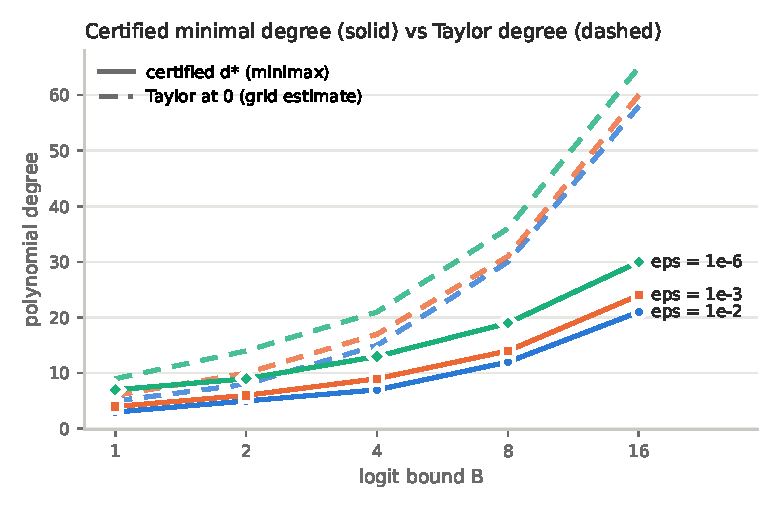
\includegraphics[width=\columnwidth]{fig_degree.pdf}\caption{Certified minimal degree d*(B, eps) for relative-error approximation of $e^x$ on [-B, B] (solid, claims [C-T-deg-\textasteriskcentered]) and the degree of the Taylor polynomial at 0 (dashed, grid estimate). Values in Table 1.}\end{figure}
\end{document}
